\documentclass[a4paper,10pt]{article}
\usepackage[utf8]{inputenc}
\usepackage[english,russian]{babel}
\usepackage{fancyhdr}
\usepackage{caption}

\usepackage{listings,longtable,amsmath,amsfonts,graphicx,tikz,tabularx}

\captionsetup{labelsep=period}
\pagestyle{fancy}

\lstset{
    basicstyle=\footnotesize,
    breakatwhitespace=false,
    breaklines=true,
    extendedchars=true,
    keepspaces=true,
    keywordstyle=\bfseries,
    numbers=left,
    numbersep=3pt,
    numberstyle=\tiny,
    showspaces=false,
    showstringspaces=false,
    showtabs=false,
    stepnumber=1,
    stringstyle=\emph,
    tabsize=2
}

\usepackage[left=1.5cm,right=1.5cm,top=2cm,bottom=1.5cm,bindingoffset=0cm]{geometry}

\captionsetup{labelsep=period}
\pagestyle{fancy}

\renewcommand{\headrulewidth}{0pt}
\fancyfoot[L] {\thepage\bf}
\fancyfoot[C] {}

\graphicspath{ {img/} }

\begin{document}
    \begin{titlepage}
        \begin{center}
            \large
            САНКТ-ПЕТЕРБУРГСКИЙ НАЦИОНАЛЬНЫЙ ИССЛЕДОВАТЕЛЬСКИЙ УНИВЕРСИТЕТ ИНФОРМАЦИОННЫХ ТЕХНОЛОГИЙ, МЕХАНИКИ И ОПТИКИ \\


            \vspace{3cm}


            Кафедра вычислительной техники
            \vspace{4cm}

            \textsc{ \textbf{Отчёт по лабораторной работе  № 1} \\
            по дисциплине <<Тестирование программного обеспечения>>\\}
            Вариант №2\\[8mm]

            \bigskip
        \end{center}
        \vspace{3cm}

        \hfill\begin{flushright}
             Студенты: Куклина М. \\ Кириллова А. 
             \vfill
             Преподаватель:
        \end{flushright}
        \vfill
        \vfill
        \vfill
        \vfill
        \vfill
        \begin{center}
            Санкт-Петербург \\2017 г.
        \end{center}
    \end{titlepage}
\newpage

\section*{Тестирование функции sec()}
	\subsection*{Тест}
        \lstinputlisting[language=java]{../firstTask/src/test/java/TestCalc.java}

\section*{Тестирование модуля Fibonacci Heap}
	\subsection*{Тест}
        \lstinputlisting[language=java]{../secondTask/src/test/java/datastructures/TestFibonacciHeap.java}
\newpage
\section*{Тестирование доменной модели для заданной области}
    \subsection*{Текст}
    	В первый момент показалось, что ничего не произошло, затем что-то засветилось на краю огромного экрана. 
        По нему ползла красная звезда величиной с тарелку, а следом за ней еще одна: бинарная звездная система.
        Затем в углу картинки возник большой полумесяц -- красный свет, переходящий в черноту -- ночная сторона планеты. 
    \subsection*{UML диаграмма}
        \begin{figure}[h!]
			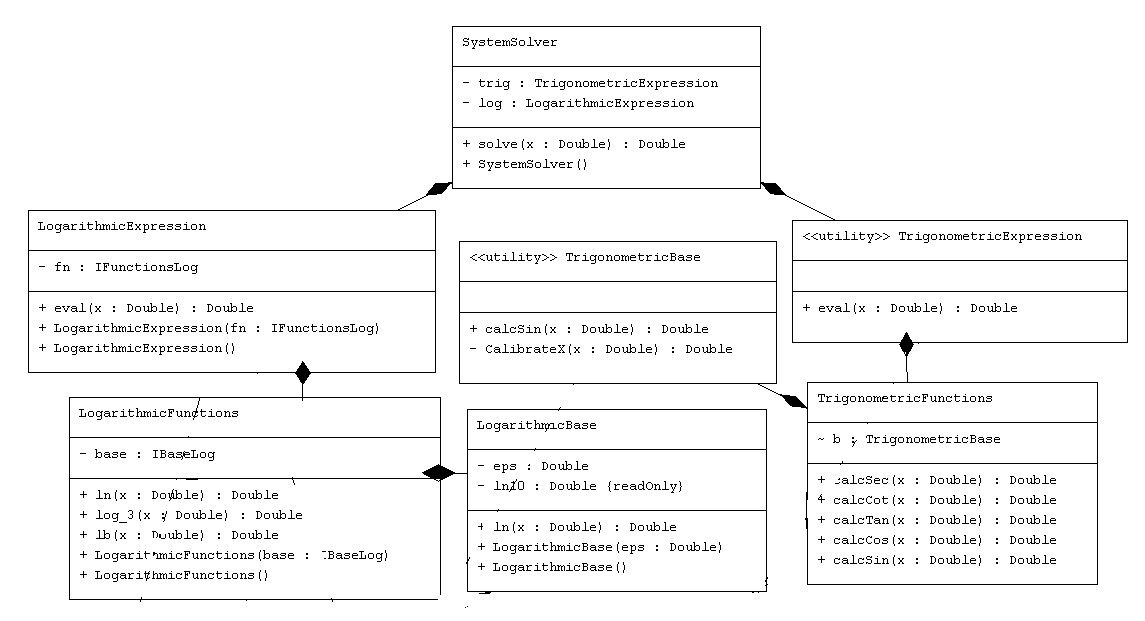
\includegraphics[scale=0.6]{../thirdTask/uml.png}
			\caption{UML диаграмма доменной модели}
		\end{figure}     
\newpage
\section*{Вывод}
    В ходе выполнения лабораторных работ было проведено тестирование разработанных программных модулей.
	При выполнении работы использовались библиотеки JUnit4 и JUnit5. Явных отличий этих библиотек
    в данной работе отмеченно не было, разве что JUnit5 имеет иную иерахию классов и модульность, 
    что делает его более гибким в сравнении с JUnit4, в котором все модули включены в платформу.
\end{document}
